\cotefile{10}
\scanpage{42}
\mspage{\handwritten{10}}
\uline{pe de présentation finie, $H_j$ un $S_j$-préschéma de présentation finie à groupe d'\unsure{opératerus|opérateurs} $G_j$. Pour que $\unsure{\mathbb{H}|H}=H_j\handwritten{\times}_{S_j}S$ soit un $S$-préschéma en espaces homogènes sous $\deleted{\unsure{H|G}}$}\margin{\figure{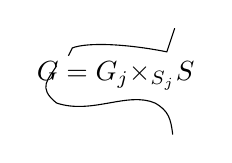
\begin{tikzpicture}[x=.5cm,y=.5cm]\node at (0,0) {$G=G_j\handwritten{\times}_{S_j}S$};\draw (1.5,1.2) -- (1.3,.6) .. controls (.3,.8) and (-.7,.85) .. (-1.1,.7) -- (-1.2,.5);\draw (-1.5,.25) .. controls (-1.7,-.1) and (-2,-.3) .. (-1.5,-.7) .. controls (-.6,-1) and (.3,-.4) .. (1,-.7) .. controls (1.35,-.9) and (1.4,-1.1) .. (1.45,-1.5);\end{tikzpicture}}}\uline{ (resp. un fibré principal homogène sous $G\inserted{\deleted{\unsure{G=G_j\times_{S_j}S}}}$\unsure{)} pour la }\uuline{topologie fidèlement plate localement de présentation finie}\uline{, il faut et il suffit qu'il existe un indice $i\handwritten{\in}I$, $i\handwritten{\geqslant}j$, tel que $H_i=H_j\handwritten{\times}_{S_j}S_i$ soit un $S_i$-préschéma en espaces homogènes sous $\deleted{\unsure{G_i}}$}\margin{\figure{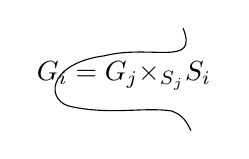
\begin{tikzpicture}[x=.5cm,y=.5cm]\node at (0,0) {$G_i=G_j\handwritten{\times}_{S_j}S_i$};\draw (1.5,1.2) .. controls (1.9,.2) and (.7,.8) .. (-.5,.5) .. controls (-2,.3) and (-2,-.7) .. (-1.3,-.8) .. controls (-.3,-1) and (.5,-.8) .. (1.2,-.9) .. controls (1.5,-1) and (1.6,-1.2) .. (1.7,-1.4);\end{tikzpicture}}}\uline{ (resp. un fibré principal homogène sous $G_i$).}

Compte tenu de (10.14) et de (EGA IV 8.8.2, 8 8.3 et 8.10.5) , \deleted{l'exp} l'énoncé résulte de l\deleted{\unsure{j|f}}a propriété concernant les morphismes \deleted{concernant}\inserted{couvrants} pour la topologie fppf rappelée en (10.0).

\figure{\begin{tikzpicture}[x=.5cm,y=.5cm]
\draw (0,11.6) .. controls (3.4,11.6) and (6.5,11.1) .. (5.1,10.2)
 .. controls (3.7,9.3) and (-1.8,7.2) .. (-.1,7.1)
 .. controls (1.9,7.0) and (4.1,7.6) .. (3.7,5.8)
 .. controls (3.5,4.8) and (2.1,3.8) .. (2.7,2.9)
 .. controls (3.4,1.9) and (5.0,1.1) .. (4.5,0);
\draw (2.45,11.7) .. controls (2.5,7.2) and (2.9,4.0) .. (3.75,.1);
\end{tikzpicture}}
% archive sheet number: 41
